% siminos/atlas/intro.tex  pdflatex atlas
% $Author$ $Date$

\begin{quotation}
    \ifdraft\color{blue}
The ``lead paragraph'' is formatted as a single paragraph before the first
section heading. Numbered references are allowed.
        \PC{
    The first paragraph of the article should be a Lead Paragraph and
    will be highlighted in the journal in boldface type. This paragraph,
    which essentially advertises the main points of the article, must
    describe in terms accessible to the nonspecialist reader the context
    and significance of the research problem studied and the importance
    of the results. The Editors will pay special attention to the clarity
    and accessibility of this paragraph, and in many cases may rewrite it
        }
    \color{black}\fi
\end{quotation}

    \PC{2012-01-03 experiment with
    \ensuremath{\hat{\ssp}}, \ensuremath{\bar{\ssp}} or \ensuremath{\tilde{\ssp}}
    as the \reducedsp\ coordinate.
    }

\section{Introduction}
\label{s:intro}
% former siminos/atlas/intro.tex

    \ifdraft\color{blue}
    \PC{
{2012-03-12} A putative outline of the paper is in
\refsect{chap:outline}.
    }
Goal: chart the \statesp\ explored by chaotic dynamics,
a curved manifold embedded in a high-dimensional \statesp.

Key notion: recurrence.
To quantify `near' need the notion of distance, or 'norm'.

Problem: evolution in time decomposes \statesp\ into spaghetti of time
orbits or trajectories. Symmetries stratify it into layers of an onion.
Need to pick a single point for each trajectory (section it) and each group orbit
(slice it).

(template)

Cover the curved manifold by the shortest-distance sections (for time
recurrence) and \slice s (for continuous transformations). In the limit of longer
and longer cycles this leads to the usual curved manifold geometry,
measured locally by Euclidean distances.
    \color{black}\fi


Over the last decade, new insights into the dynamics of moderate
\Reynolds\ turbulent flows have been gained through visualizations of
their $\infty$-dimensional \statesp s by means of dynamically invariant,
representation independent coordinate frames\rf{GHCW07} constructed from
physically prominent unstable coherent states, hereafter referred to {\em
\template s}.
    \DB{2012-04-10}{
    Since we are talking about coherent structures in the context
    of turbulence, should we distinguish `exact' coherent structures from
    Lagrangian coherent structures, POD modes, etc?
    }
The most recent advance within this bold new framework is
the first determination of \rpo s that in part shape turbulence observed
in pipe flows\rf{ACHKW11}. Navigating and charting the geometry of these
extremely high-dimensional \statesp s necessitates a reexamination of two
of the basic tools of the theory of dynamical systems: Poincar\'e
sections and symmetry
reduction\rf{rowley_reconstruction_2000,BeTh04,SiCvi10,FrCv11}. We strive
here to explain the key geometrical ides in simple but illustrative
settings, eschewing the fluid dynamical and group theoretical
technicalities.
%    \PC{DB: I thought
%    the method of slices was not in everybody's bag of tricks. We also
%    discuss some further methods, at least as per the outline.
%    Predrag: agreed}


%%%%%%%%%%%%%%%%%%%%%%%%%%%%%%%%%%%%%%%%%%%%%%%%%%%%%%%%%%%%%%%%%%%%%
\begin{figure}
   \centering
  \setlength{\unitlength}{0.20\textwidth}
(a)~~~
  \begin{picture}(1,0.98239821)%
    \put(0,0){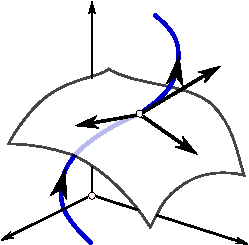
\includegraphics[width=\unitlength]{A28tangent3}}%
    \put(0.91612064,0.70682767){\color[rgb]{0,0,0}\makebox(0,0)[lb]{\smash{$\vel$}}}%
    \put(0.48698745,0.90266503){\color[rgb]{0,0,0}\makebox(0,0)[lb]{\smash{$\ssp(\zeit)$}}}%
    \put(0.2624318,0.5347756){\color[rgb]{0,0,0}\makebox(0,0)[lb]{\smash{$\groupTan_1$}}}%
    \put(0.80471037,0.38188675){\color[rgb]{0,0,0}\makebox(0,0)[lb]{\smash{$\groupTan_2$}}}%
    \put(0.538343,0.25344355){\color[rgb]{0,0,0}\makebox(0,0)[lb]{\smash{$\LieEl\ssp$}}}%
    \put(0.47864531,0.56060893){\color[rgb]{0,0,0}\makebox(0,0)[lb]{\smash{$\ssp$}}}%
  \end{picture}%
~~(b)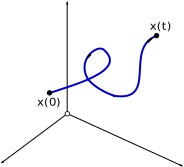
\includegraphics[width=0.20\textwidth]{A27traj}
\\
(c)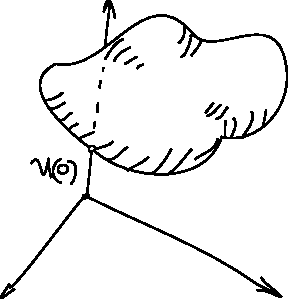
\includegraphics[width=0.20\textwidth]{A27gOrbit}
(d)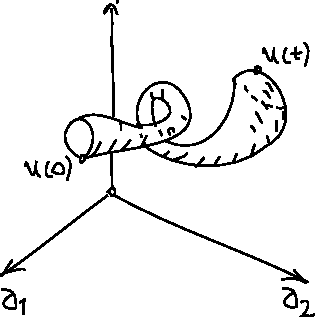
\includegraphics[width=0.20\textwidth]{A27wurst}
   \caption{\label{fig:A27wurst}
   (a)
In presence of $N$-continuous parameter symmetry, each \statesp\ point
$\ssp$ owns $(N\!+\!1)$ tangent vectors: one $\vel(\ssp)$ along the time
flow $\ssp(\zeit)$, and the $N$ group tangents  $\groupTan_1(\ssp), \,
\groupTan_2(\ssp) ,\,\cdots, \groupTan_N(\ssp)$ along infinitesimal
symmetry shifts, tangent to the group orbit $\LieEl\ssp$.
    (b)
Trajectory.
    (c)
Group orbit.
    (d)
Wurst.
}
\end{figure}
%%%%%%%%%%%%%%%%%%%%%%%%%%%%%%%%%%%%%%%%%%%%%%%%%%%%%%%%%%%%%%%%%%%%%

A flow $\map^t$ and the \statesp\ $\pS$ on which the flow acts comprise a
{\em dynamical system}.
If a group $\Group$ of continuous transformations acts on a continuous
time flow, each \statesp\ point owns a set of tangent vectors,
\reffig{fig:A27wurst}\,(a). Integrated globally, the velocity vector
$\vel(\ssp)$ traces out the the {\em trajectory} $\flow{\zeit}{\ssp}$,
\reffig{fig:A27wurst}\,(b), and the continuous transformations trace out
the \emph{group orbit}
\(
\pS_\ssp = \{\LieEl\,\ssp \mid \LieEl \in {\Group}\}
% \,,\qquad \pS_\ssp \subset \pS
\,,
\) %ee{sspOrbit}
\reffig{fig:A27wurst}\,(c). Together they trace out a complicated smooth
manifold (hereafter affectionately referred to as the {\em wurst}, see
\reffig{fig:A27wurst}\,(d) and \reffig{fig:sliceimage}), that we shall
learn how to slice in \refsect{s:slice}.
A flow is said to have symmetry $\Group$ if the form of evolution
equations $\dot{\ssp} = \vel(\ssp)$ is left invariant,
\(
\vel(\ssp)=\LieEl^{-1} \, \vel(\LieEl \, \ssp)
\,,\qquad \mbox{for all }
\,,
\) %ee{eq:FiniteRot}
by the set of transformations $\LieEl \in {\Group}$. While the flow
equations are invariant under $\Group$, their solutions typically are
not.

After some observations of a given turbulent flow, one can identify a set
of \emph{\template s}\rf{rowley_reconstruction_2000}, {points}
$\slicep{}^{(j)}$, $j=1,2,\cdots$ in the \statesp\ $\pS$, which are the
dynamically most important unstable {\recurrStr s} of the flow.


\begin{itemize}

    \ifdraft\color{blue}
  \item
        norms; minimal distance
  \item section {\PoincS} vs slice \pSRed

  \item
dynamical system  with symmetry \Group\ vs reduced dynamics
$\{\pSRed,\mapRed^t\}$ , hereafter affectionately referred to as the {\em
sliced wurst}, to be sliced in what follows.
  \item strobing $\sim$ method of connections
  \item reduction vs projection
    \color{black}\fi
\end{itemize}

Our goals here are two-fold:
(i) In \refsect{s:cut} we review the method of Poincar\'e sections, with
    emphasis on aspects applicable to high-dimensional flows: construction of
    multiple local linear sections and determination of their borders, and then in
(ii) \refsect{s:slice} show how the same set of tools applied to
    reduction of continuous symmetries enables us to commence a
    systematic charting of the long-time dynamics of high-dimensional
    flows with continuous symmetries.
